\documentclass{beamer}

\usepackage[utf8]{inputenc}
\usepackage[T1]{fontenc}
\usepackage{textcomp}
\usepackage{times}

%\usetheme[sky-200]{UiO}
\usetheme{Frankfurt}
\usecolortheme{orchid}

\usepackage{color}

\title{How social media affect FOSS}
\subtitle{INF5780 Project 2}
\author{{John Rongved} \and {Lars Tveito} \and {Kristian A. Hiorth}}
\date{November 13, 2014}

\institute{Department of Informatics\\University of Oslo}

% fits the presentation to the window when first displayed
\hypersetup{pdfstartview={Fit}}

\AtBeginSubsection[]
{
  \begin{frame}<beamer>{Outline}
    \tableofcontents[currentsection,currentsubsection]
  \end{frame}
}

\newcommand{\coloreddot}[1][black]{\Large\textcolor{#1}{\ensuremath\bullet}}
\setbeamertemplate{caption}{\raggedright\insertcaption\par}

\begin{document}


\begin{frame}
  %\maketitle
  \titlepage
\end{frame}

\begin{frame}{Outline}
  \tableofcontents{}
\end{frame}

\section{Motivation}

\subsection{Social Media}

\begin{frame}
  \frametitle{The project}
  ns-3 is a pretty popular network simulator. {\small
    \url{http://www.nsnam.org}}

  \begin{itemize}
  \item Successor to the prolific ns-2 simulator.
  \item GPLv2 license.
  \item Mostly academic/research users, many of whom contribute back to
    the project
  \end{itemize}
\end{frame}

\begin{frame}
  \frametitle{GitHub vs Sourceforge}
  \begin{figure}
    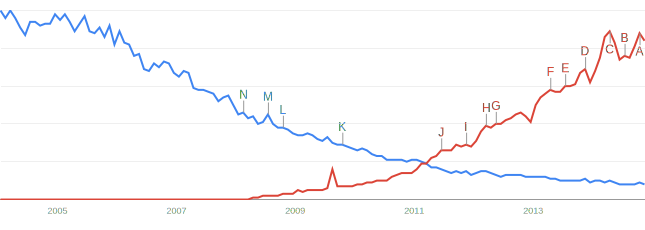
\includegraphics[width=\textwidth]{sourceforge-github.pdf} \\
    \caption{\coloreddot[red] Github \hspace{2em} \coloreddot[blue] Sourceforge}
    \end{figure}
\end{frame}


\section{Related work}

\subsection{Social coding}

\begin{frame}
  \frametitle{Premise}

  \begin{columns}[T]
    \begin{column}{.5\textwidth}
      \begin{itemize}

      \item
        
        \uncover<2->{

        \item

        \item
        }

      \end{itemize}

      \uncover<3->{
        $\Longrightarrow$ API incompatibility
      }
    \end{column}
    \begin{column}{.5\textwidth}
      %\includegraphics[width=\textwidth]{pyviz_shell.png}
    \end{column}
  \end{columns}
\end{frame}

\subsection{Social Q \&{} A}

\subsection{Social news}


\section{Discussion}

\subsection{Shizz}

\begin{frame}
  Shoozial mediaz da bomb, man.
\end{frame}

\section*{Summary}

\begin{frame}
  We showed dem mediaz be sozial.

  
  \pause
  \vskip0pt plus.5fill

  Questions?
\end{frame}

\end{document}
